\chapter{Implementacija i korisničko sučelje}
		
		
		\section{Korištene tehnologije i alati}
			
			Tim uspješno komunicira putem aplikacija Discord i WhatsApp, omogućavajući efikasnu i brzu razmjenu informacija. 
			
			UML dijagrami napisani su u okruženju AstahUML. Koristimo ih za vizualizaciju i analizu softverskog rješenja, što pomaže boljem razumijevanju arhitekture i funkcionalnosti sustava.
			
			U procesu razvoja koristimo Git za upravljanje verzijama koda, s udaljenim repozitorijem na GitHubu. Ovo omogućava timsku suradnju, praćenje promjena i povratak na prethodne verzije koda po potrebi. Korištena razvojna okruženja su IntelliJ za programski jezik Java i WebStorm za p. jezik JavaScript, čime smo osigurali snažne alate za razvoj i debugiranje aplikacije. Što se tiče samog softverskog rješenja, frontend aplikacija je napisana u JavaScriptu, koristeći biblioteku ReactJS i Node.js za poslužitelja web aplikacije. Backend je napisan u Java Spring framework-u, time je pružena stabilnost serverskom dijelu.
			
			Za registraciju koristimo Google reCAPTCHA API kako bi povećavali sigurnost aplikacije. Sve slike koje koristimo skladištimo na Firebase Cloud platformi, pružajući pouzdanu infrastrukturu za upravljanje multimedijskim sadržajem. 
			U fazi razvoja koristimo H2 bazu podataka, dok aplikacija u pogonu koristi udaljenu PostgreSQL instancu pruženu od strane Render platforme. Pogon aplikacije vršimo putem Render platforme, što omogućava jednostavan i efikasan proces.
			
			Za pisanje dokumentacije koristimo TexStudio okruženje, koje podržava LaTeX jezik. Ova kombinacija omogućava strukturirano i profesionalno dokumentiranje rješenja. 
			
			Sve ove tehnologije i alati zajedno čine tim sposobnim za efikasan razvoj, održavanje i dokumentiranje softverskog rješenja.
			
			\eject 
		
	
		\section{Ispitivanje programskog rješenja}
			
			\textbf{\textit{dio 2. revizije}}\\
			
			 \textit{U ovom poglavlju je potrebno opisati provedbu ispitivanja implementiranih funkcionalnosti na razini komponenti i na razini cijelog sustava s prikazom odabranih ispitnih slučajeva. Studenti trebaju ispitati temeljnu funkcionalnost i rubne uvjete.}
	
			
			\subsection{Ispitivanje komponenti}
			\textit{Potrebno je provesti ispitivanje jedinica (engl. unit testing) nad razredima koji implementiraju temeljne funkcionalnosti. Razraditi \textbf{minimalno 6 ispitnih slučajeva} u kojima će se ispitati redovni slučajevi, rubni uvjeti te izazivanje pogreške (engl. exception throwing). Poželjno je stvoriti i ispitni slučaj koji koristi funkcionalnosti koje nisu implementirane. Potrebno je priložiti izvorni kôd svih ispitnih slučajeva te prikaz rezultata izvođenja ispita u razvojnom okruženju (prolaz/pad ispita). }
			
			
			
			\subsection{Ispitivanje sustava}
			
			 \textit{Potrebno je provesti i opisati ispitivanje sustava koristeći radni okvir Selenium\footnote{\url{https://www.seleniumhq.org/}}. Razraditi \textbf{minimalno 4 ispitna slučaja} u kojima će se ispitati redovni slučajevi, rubni uvjeti te poziv funkcionalnosti koja nije implementirana/izaziva pogrešku kako bi se vidjelo na koji način sustav reagira kada nešto nije u potpunosti ostvareno. Ispitni slučaj se treba sastojati od ulaza (npr. korisničko ime i lozinka), očekivanog izlaza ili rezultata, koraka ispitivanja i dobivenog izlaza ili rezultata.\\ }
			 
			 \textit{Izradu ispitnih slučajeva pomoću radnog okvira Selenium moguće je provesti pomoću jednog od sljedeća dva alata:}
			 \begin{itemize}
			 	\item \textit{dodatak za preglednik \textbf{Selenium IDE} - snimanje korisnikovih akcija radi automatskog ponavljanja ispita	}
			 	\item \textit{\textbf{Selenium WebDriver} - podrška za pisanje ispita u jezicima Java, C\#, PHP koristeći posebno programsko sučelje.}
			 \end{itemize}
		 	\textit{Detalji o korištenju alata Selenium bit će prikazani na posebnom predavanju tijekom semestra.}
			
			\eject 
		
		
		\section{Dijagram razmještaja}
			
			\textbf{\textit{dio 2. revizije}}
			
			 \textit{Potrebno je umetnuti \textbf{specifikacijski} dijagram razmještaja i opisati ga. Moguće je umjesto specifikacijskog dijagrama razmještaja umetnuti dijagram razmještaja instanci, pod uvjetom da taj dijagram bolje opisuje neki važniji dio sustava.}
			
			\eject 
		
		\section{Upute za puštanje u pogon}
		
		Aplikacija je puštena u pogon koristeći alat Render. Koristeći korisničko sučelje koje Render pruža treba kreirati instancu baze podataka, instancu za web servis backenda te instancu za web servis frontenda aplikacije. Prvo treba kreirati bazu podataka PostgreSQL.
			
			\begin{figure}[H]
				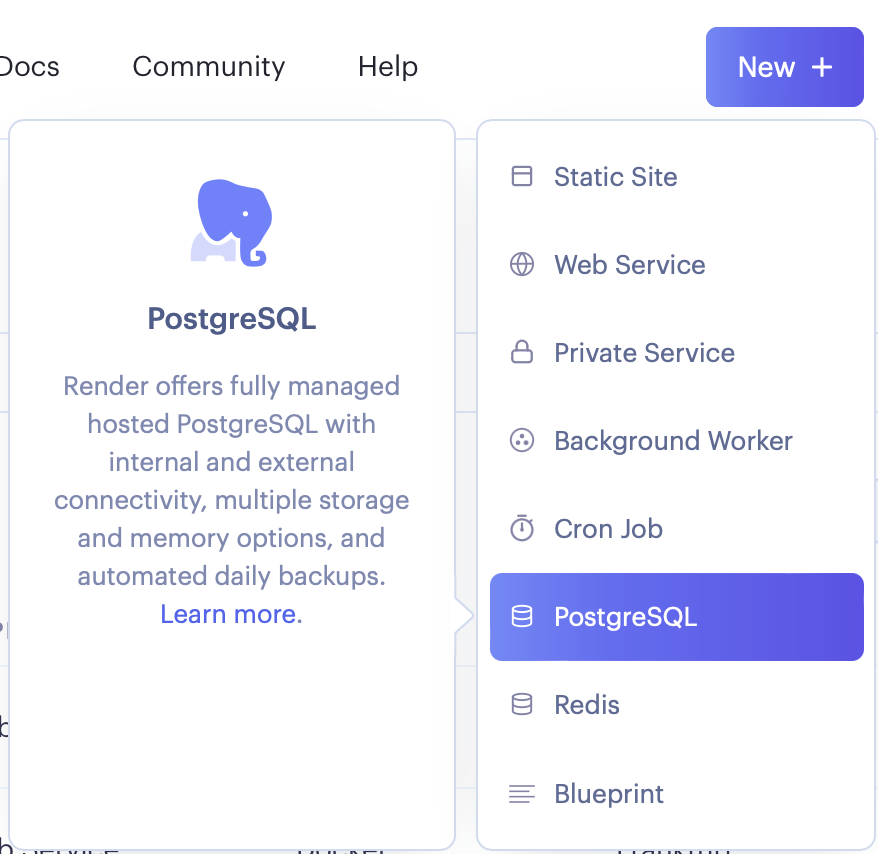
\includegraphics[scale=0.3]{slike/deploy/database1.png} %veličina slike u odnosu na originalnu datoteku i pozicija slike
				\centering
				\caption{Izbornik za stvaranje nove baze podataka}
				\label{fig:promjene}
			\end{figure}
			
			Potrebno je upisati ime baze, odabrati regiju poslužitelja instance i označiti tip instance koji će se koristiti.
			\begin{figure}[H]
				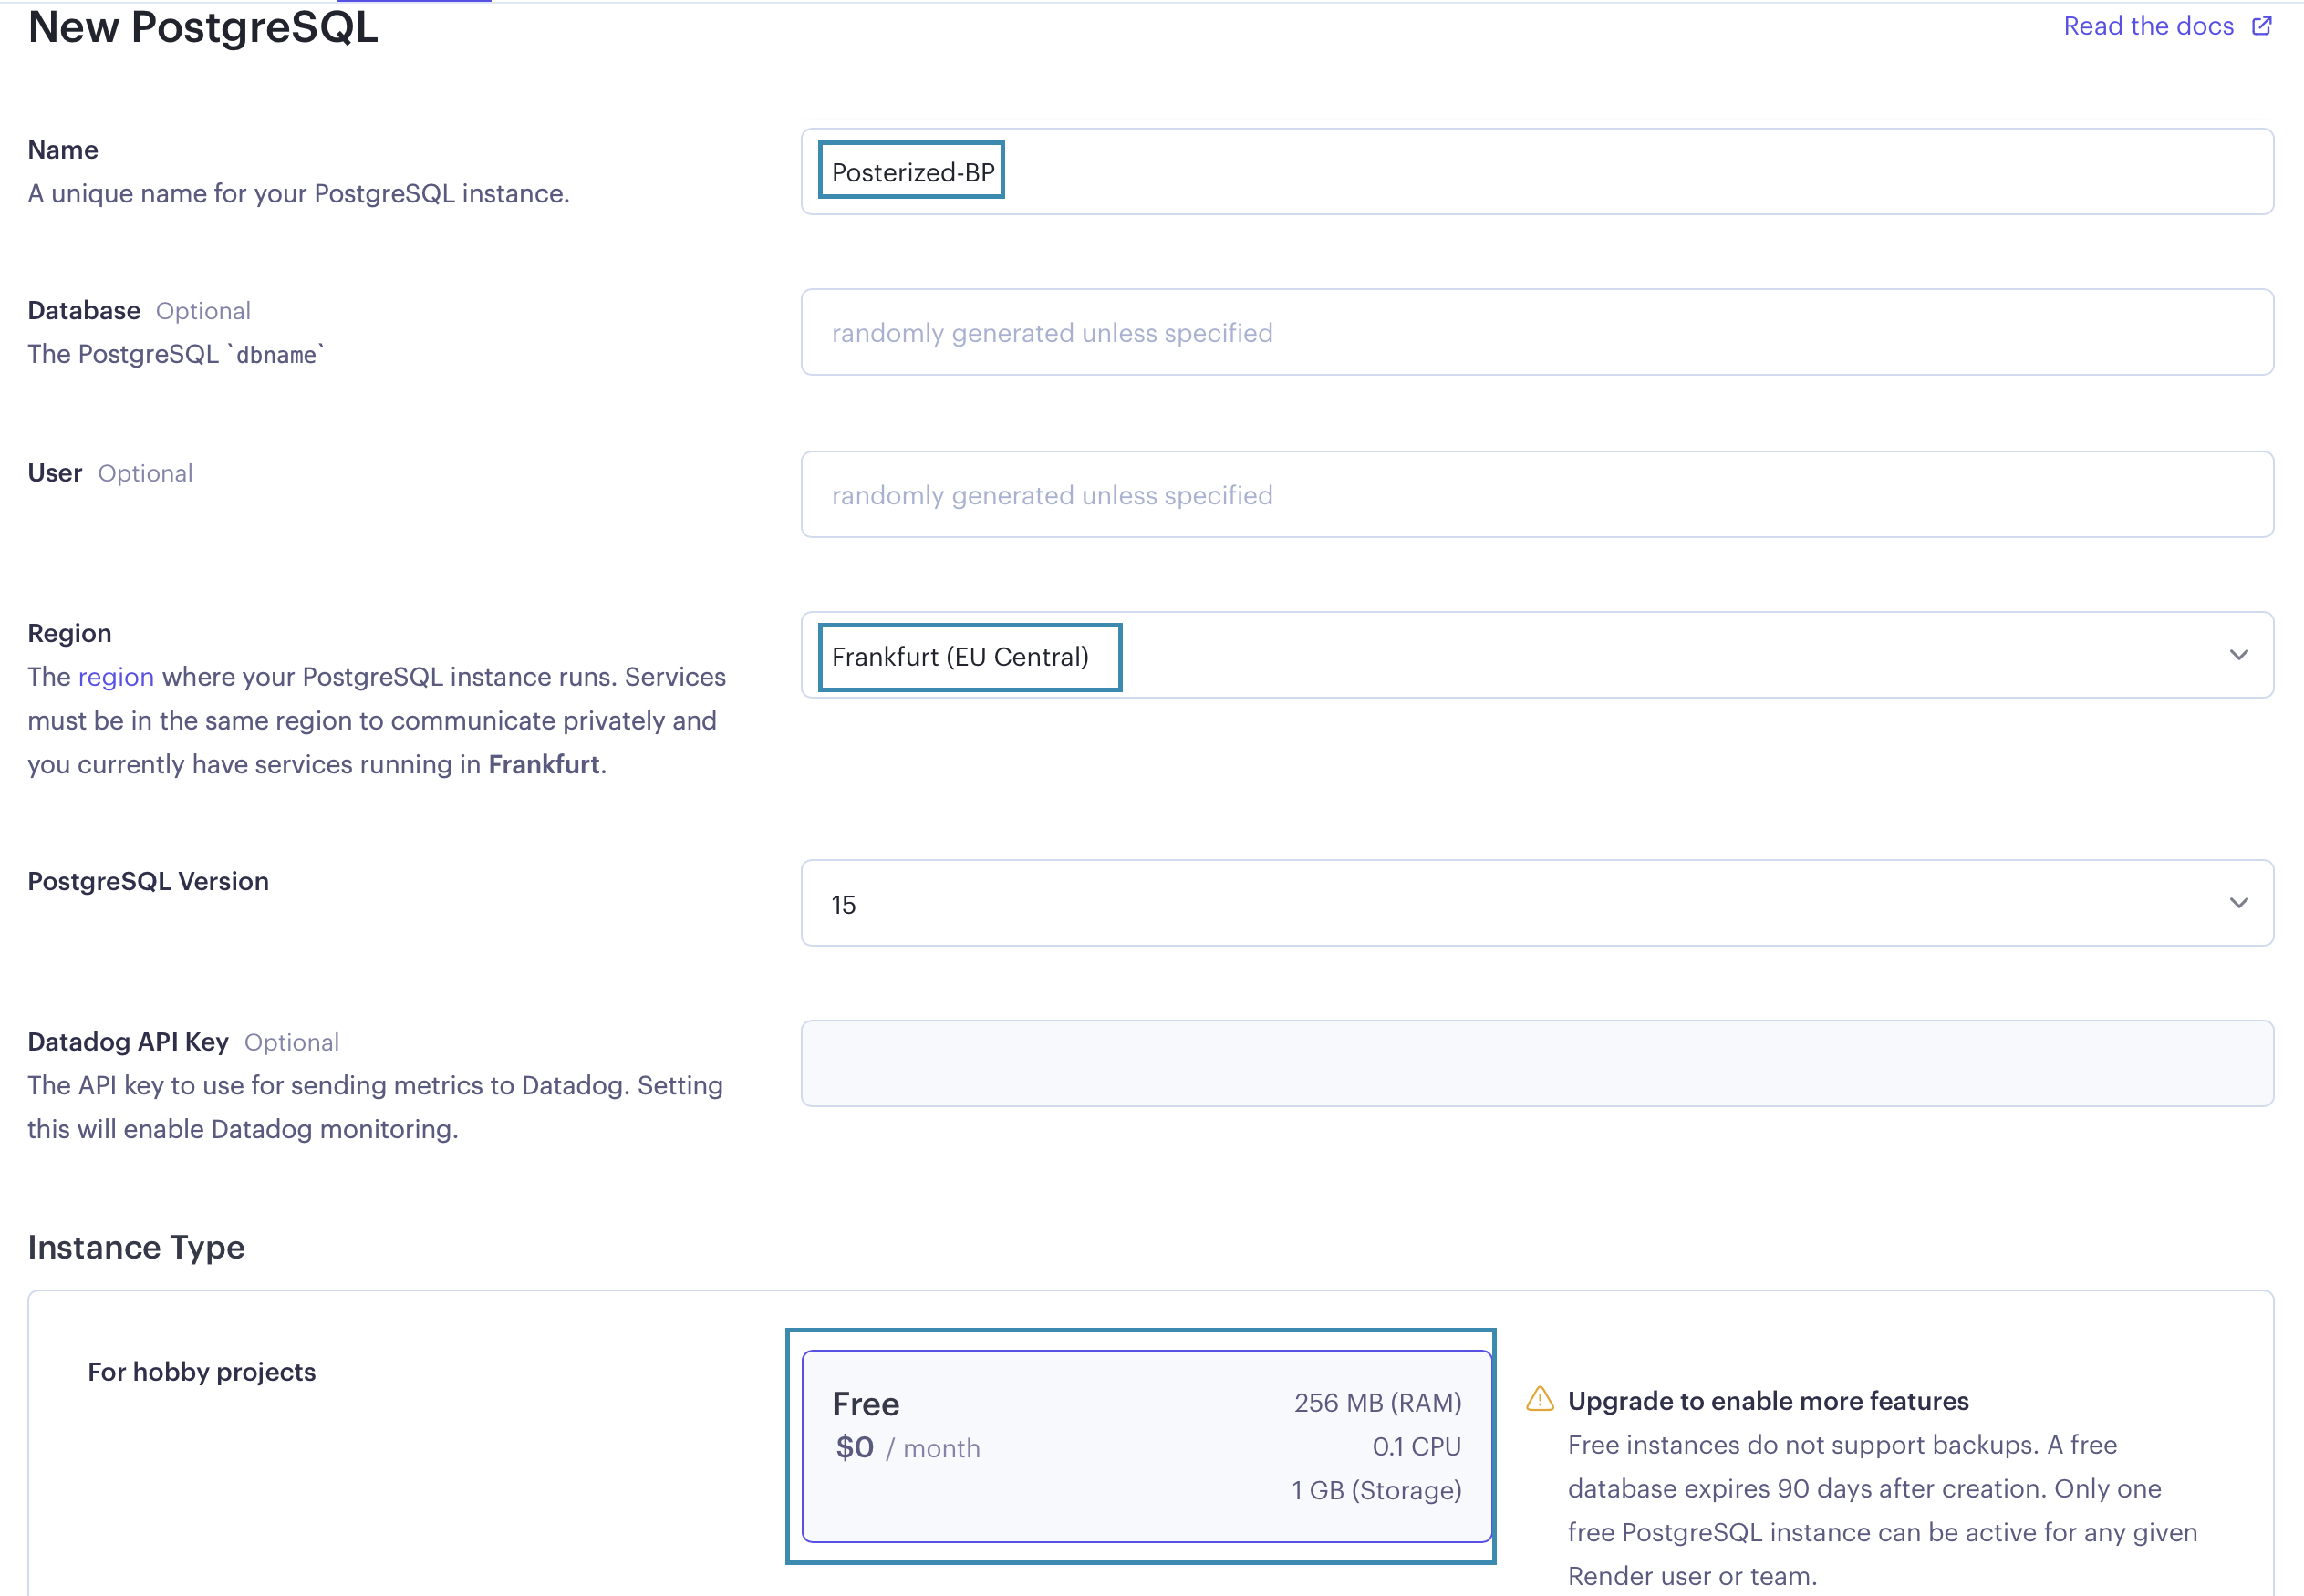
\includegraphics[scale=0.3]{slike/deploy/database2.png} %veličina slike u odnosu na originalnu datoteku i pozicija slike
				\centering
				\caption{Stvaranje nove baze podataka}
				\label{fig:promjene}
			\end{figure}
			Nakon ovih koraka treba pokrenuti stvaranje pritiskom na tipku "Create".
			
			Pokazuje se prozor u kojemu su navedeni osnovni podatci o bazi kao ime, verzija, regija, prostor za pohranu, API ključ, itd.
			\begin{figure}[H]
				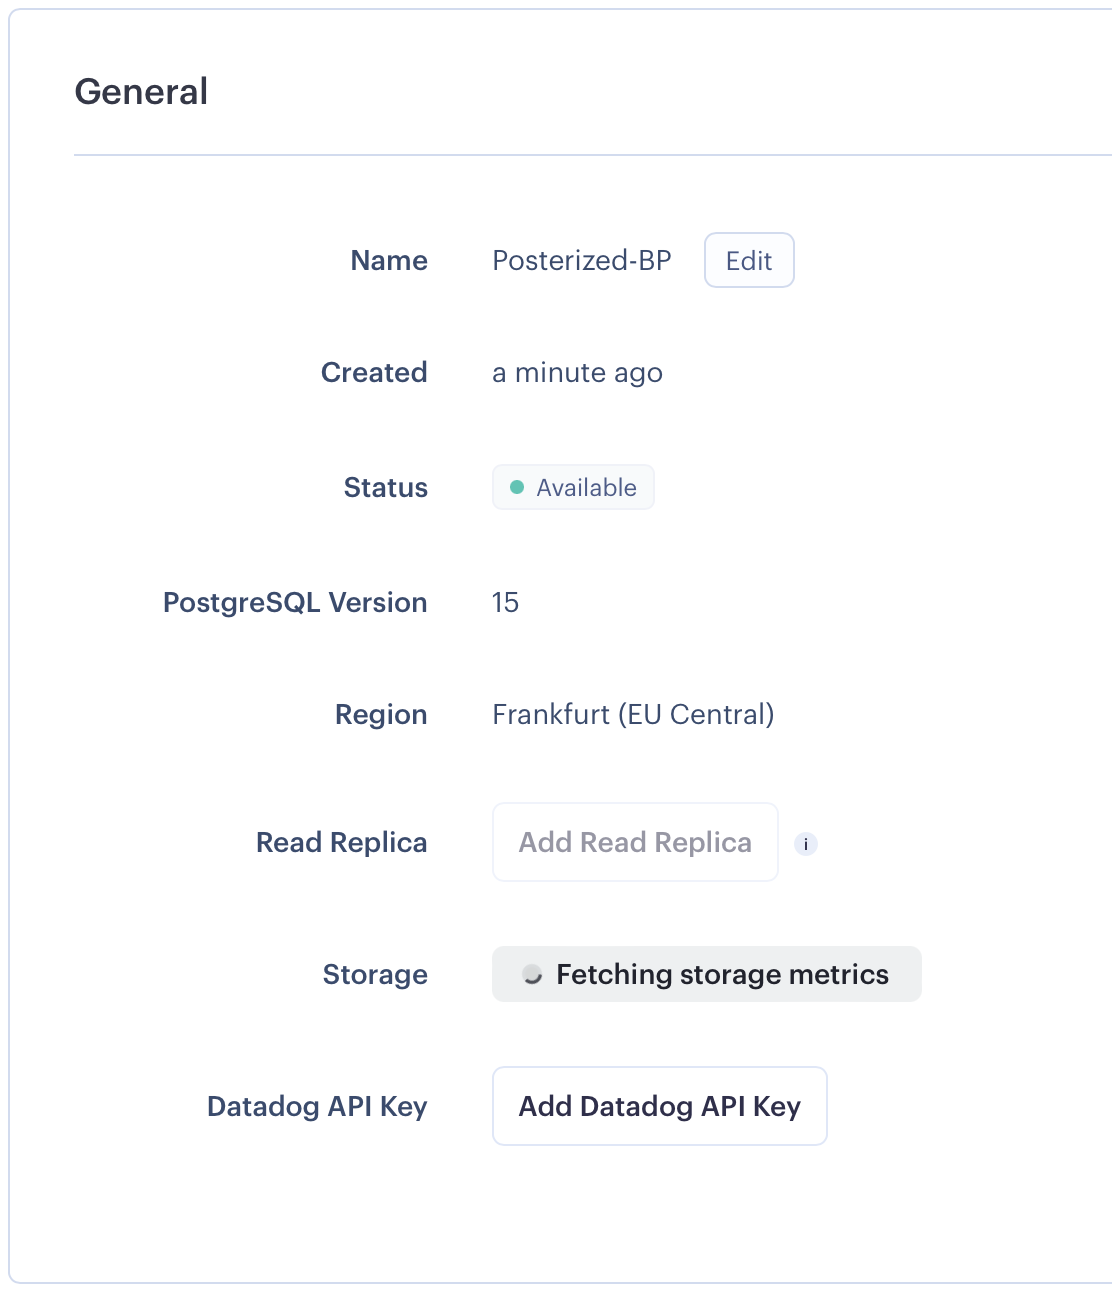
\includegraphics[scale=0.3]{slike/deploy/database3.png} %veličina slike u odnosu na originalnu datoteku i pozicija slike
				\centering
				\caption{Osnovni podatci o statusu baze podataka}
				\label{fig:promjene}
			\end{figure}
			
			Kad je baza uspješno kreirana, potrebno je uzeti podatke koje treba dati backendu aplikacije. Ti podatci se nalaze u poljima \textit{Hostname}, \textit{Port}, \textit{Database}, \textit{Username}, \textit{Password} i \textit{External Database URL}.
			\begin{figure}[H]
				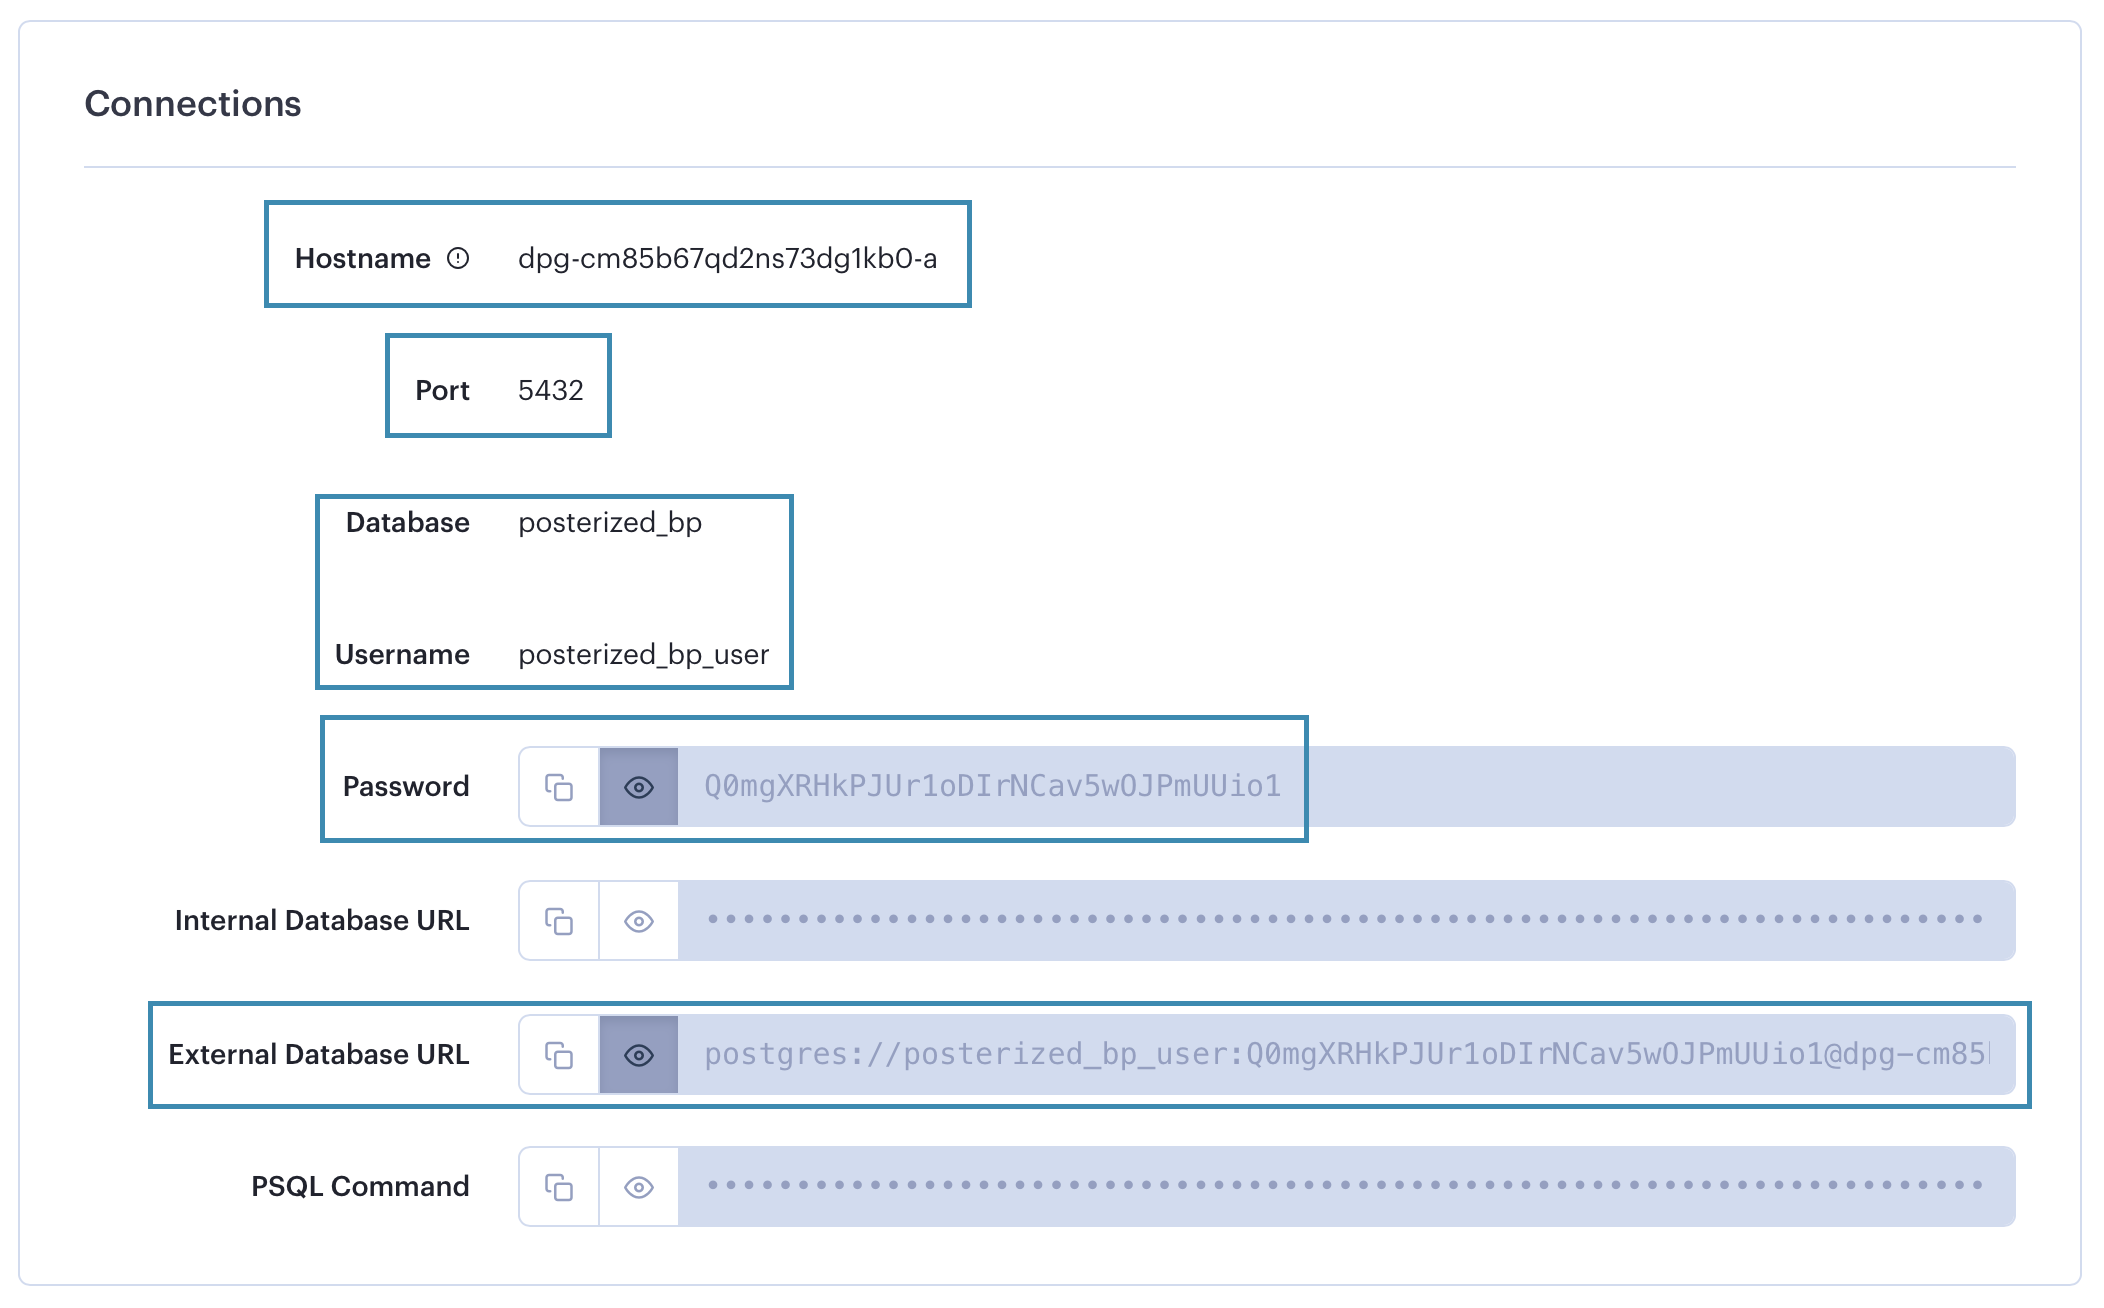
\includegraphics[scale=0.4]{slike/deploy/database4.png} %veličina slike u odnosu na originalnu datoteku i pozicija slike
				\centering
				\caption{Podatci za pristupanje bazi podataka}
				\label{fig:promjene}
			\end{figure}
			
			\pagebreak
			 Za kreiranje backend web servisa potrebno je prvo napraviti pripremu pa automatsko kreiranje web servisa iz GitHub repozitorija. U projektu razvojnog okruženja treba dodati port servera, kontekstnu putanju, podatke za pristup bazi upisati u označeni prozor te izbrisati aktivni dev profil.
			\begin{figure}[H]
				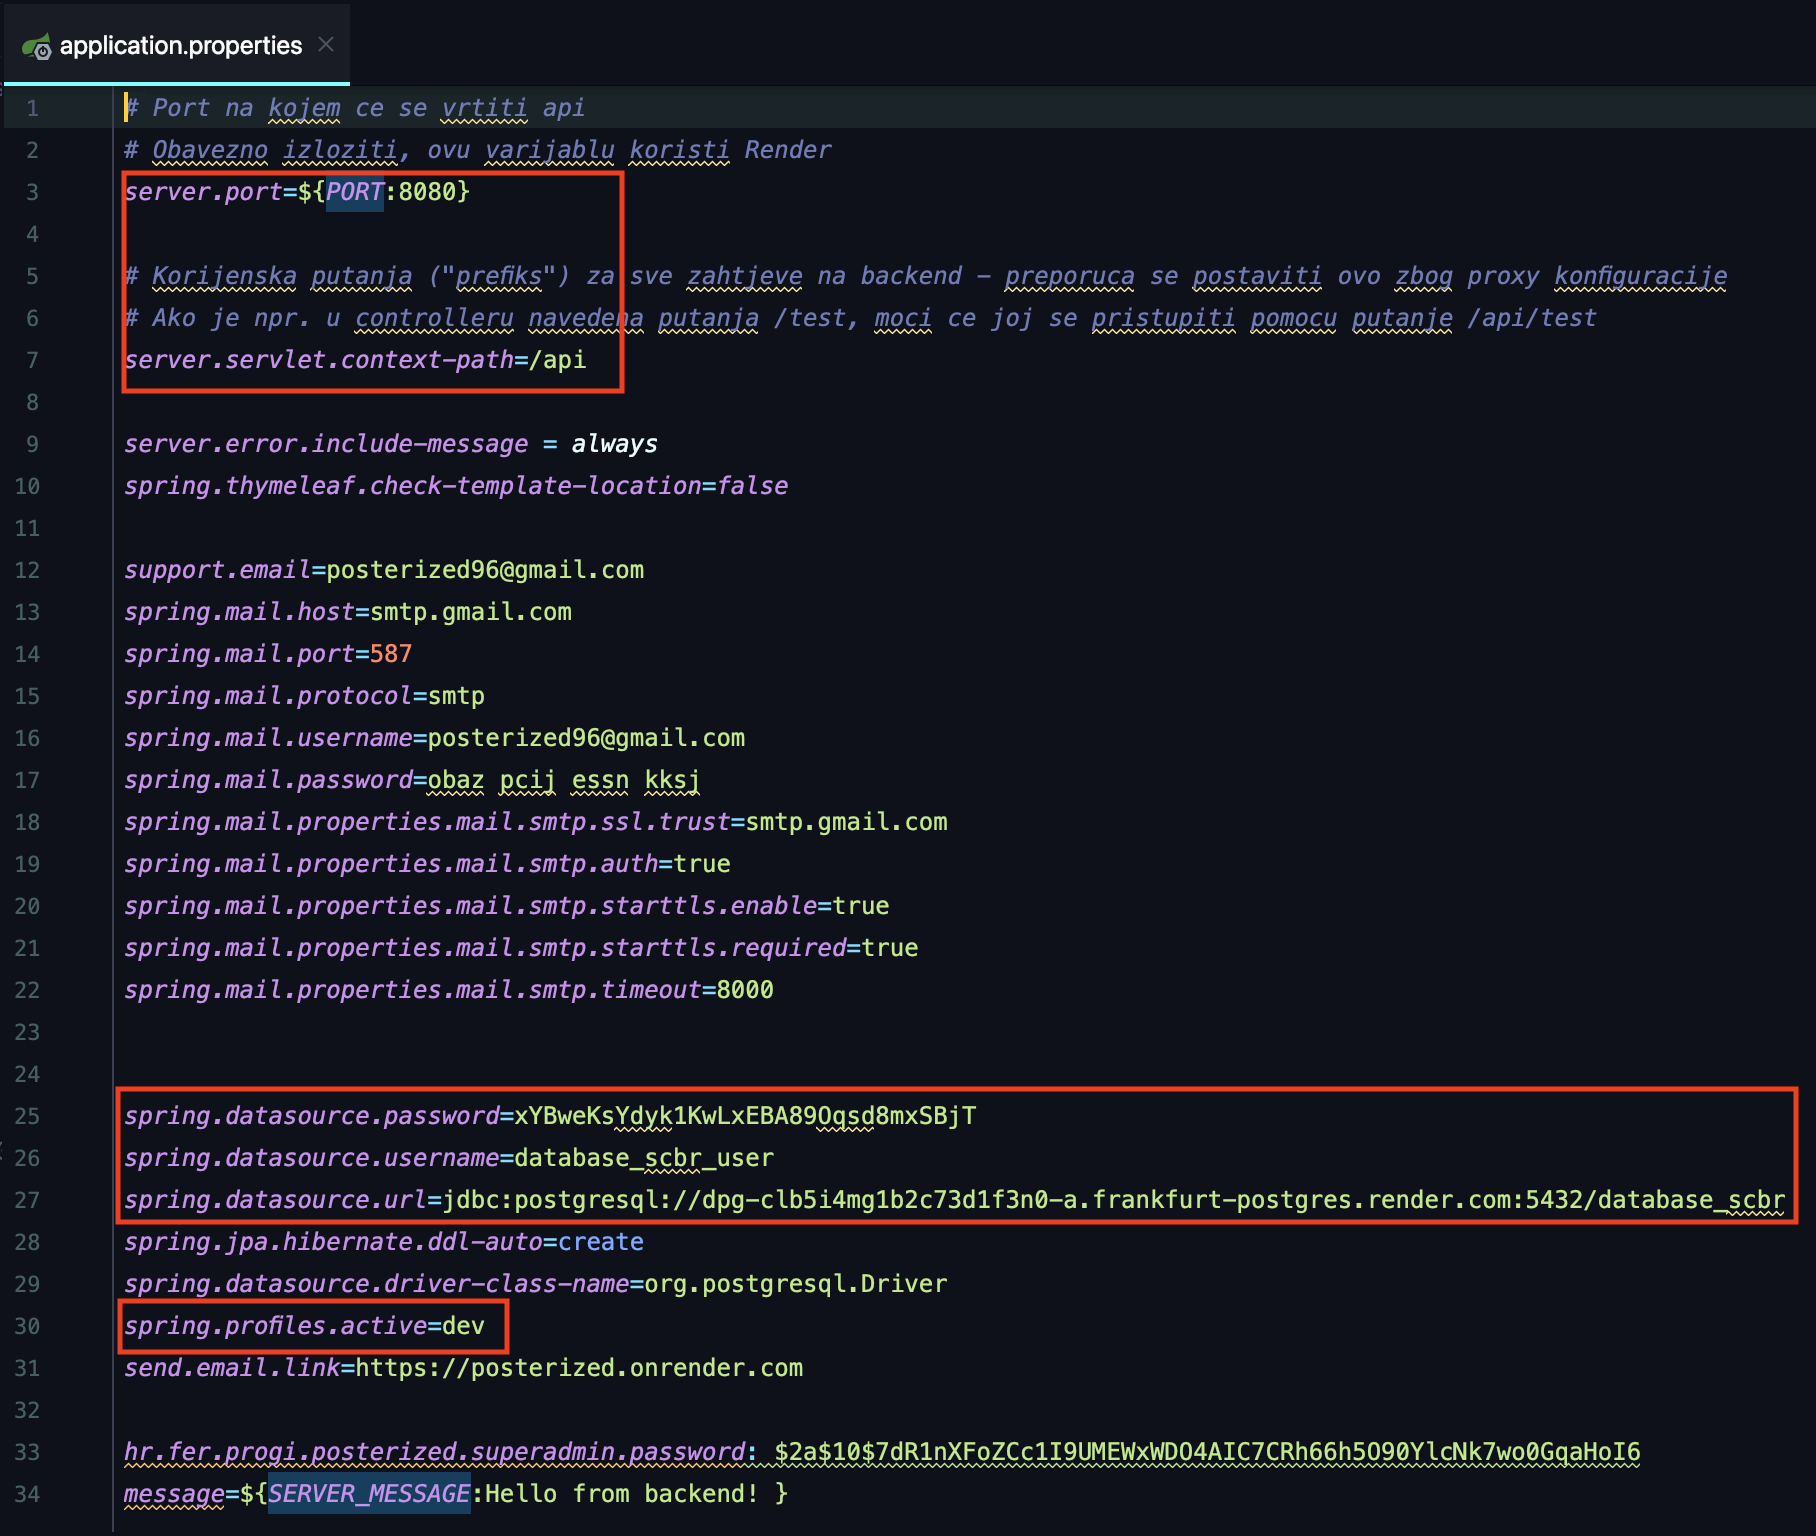
\includegraphics[scale=0.4]{slike/deploy/backend8.png} %veličina slike u odnosu na originalnu datoteku i pozicija slike
				\centering
				\caption{Datoteka \textit{application.properties}}
				\label{fig:promjene}
			\end{figure}
			U projekt je potrebno ubaciti odgovarajući \textit{Dockerfile} na putanju \textit{./posterized-backend/docker/maven} koja je prikazana stablom.
			\begin{figure}[H]
				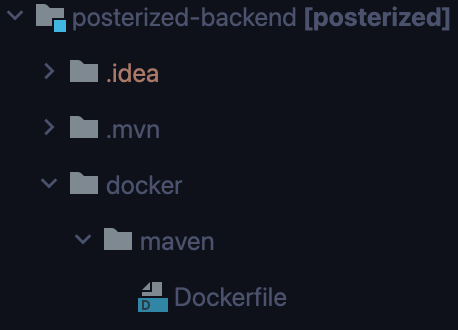
\includegraphics[scale=0.8]{slike/deploy/backend7.png} %veličina slike u odnosu na originalnu datoteku i pozicija slike
				\centering
				\caption{Stablo u kojem se nalazi \textit{Dockerfile}}
				\label{fig:promjene}
			\end{figure}
			
			\pagebreak
			Kreiranje web servisa se pokreće iz Renderovog izbornika.
			\begin{figure}[H]
				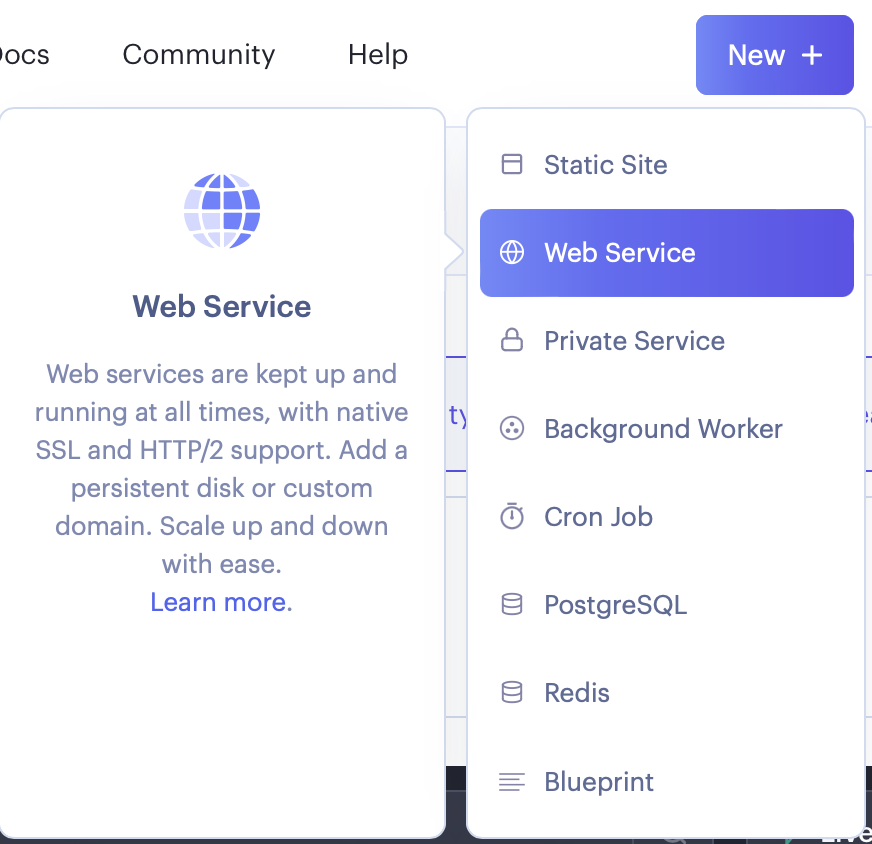
\includegraphics[scale=0.4]{slike/deploy/backend00.png} %veličina slike u odnosu na originalnu datoteku i pozicija slike
				\centering
				\caption{Izbornik za kreiranje web servisa}
				\label{fig:promjene}
			\end{figure}
			Potrebno je povezati GitHub repozitorij s Renderom. Označiti "Build and deploy from a Git repository" i kliknuti "Next".
			\begin{figure}[H]
				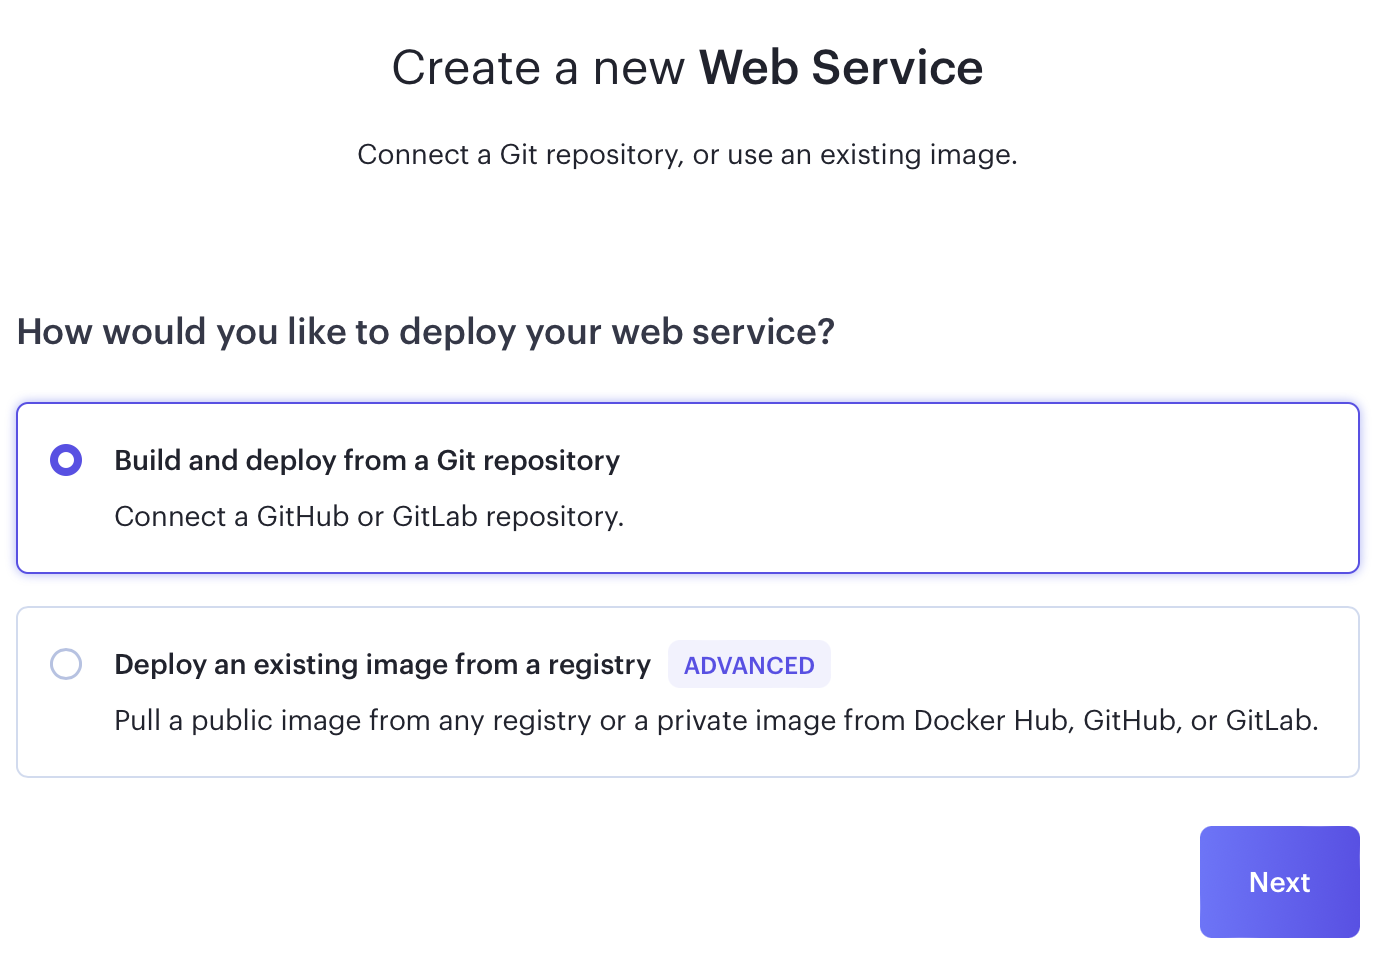
\includegraphics[scale=0.4]{slike/deploy/backend1.png} %veličina slike u odnosu na originalnu datoteku i pozicija slike
				\centering
				\caption{Kreiranje web servisa - povezivanje s udaljenim repozitorijem}
				\label{fig:promjene}
			\end{figure}
			\pagebreak
			Kliknuti "Connect GitHub", prijaviti se u račun, odobriti autorizaciju i kliknuti "Connect".
			\begin{figure}[H]
				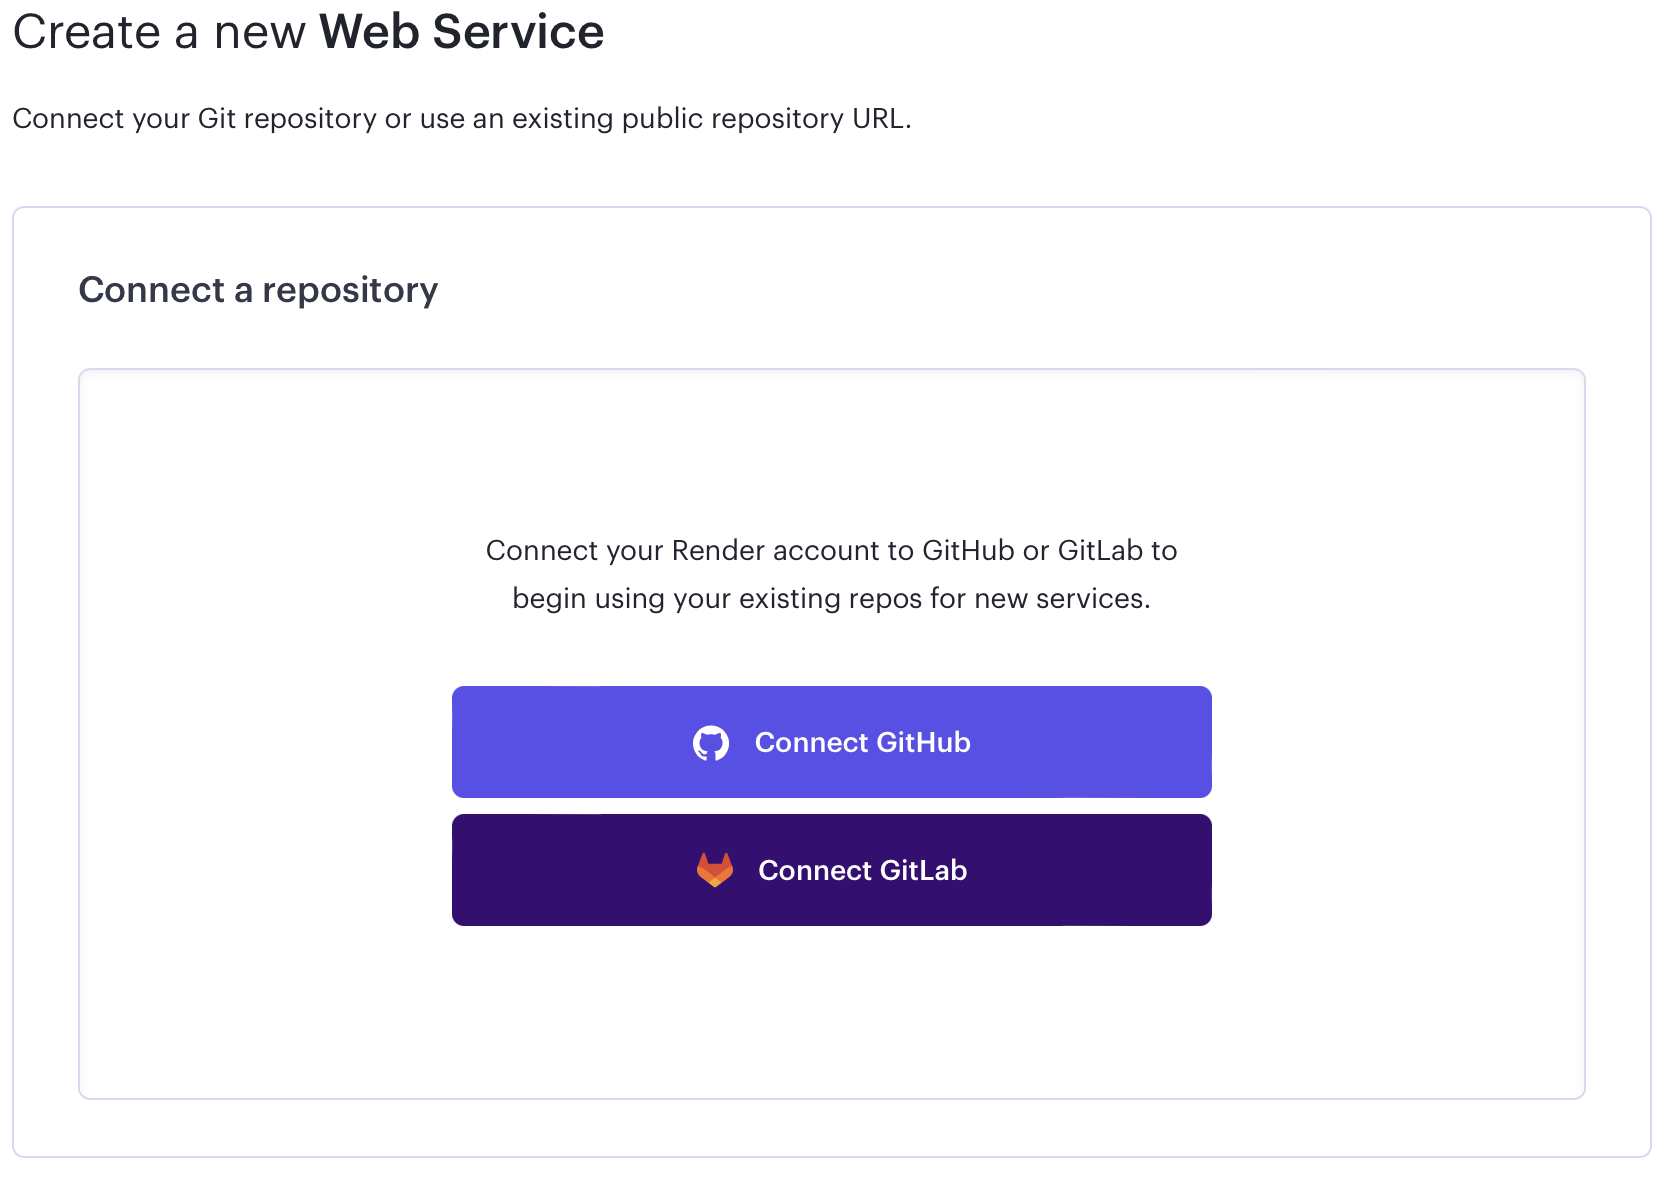
\includegraphics[scale=0.25]{slike/deploy/backend2.png} %veličina slike u odnosu na originalnu datoteku i pozicija slike
				\centering
				\caption{Povezivanje s repozitorijem}
				\label{fig:promjene}
			\end{figure}
			
			\begin{figure}[H]
				
\includegraphics[scale=0.3]{slike/deploy/backend3.png} %veličina slike u odnosu na originalnu datoteku i pozicija slike
				\centering
				\caption{Pronađeni repozitorij}
				\label{fig:promjene}
			\end{figure}
			Upisati ime servisa i odabrati regiju koja je najbliža našoj lokaciji.  Pod \textit{Branch} odabrati master i upisati ime mape projekta. Odabrati tip instance koji će se koristiti.
			\begin{figure}[H]
				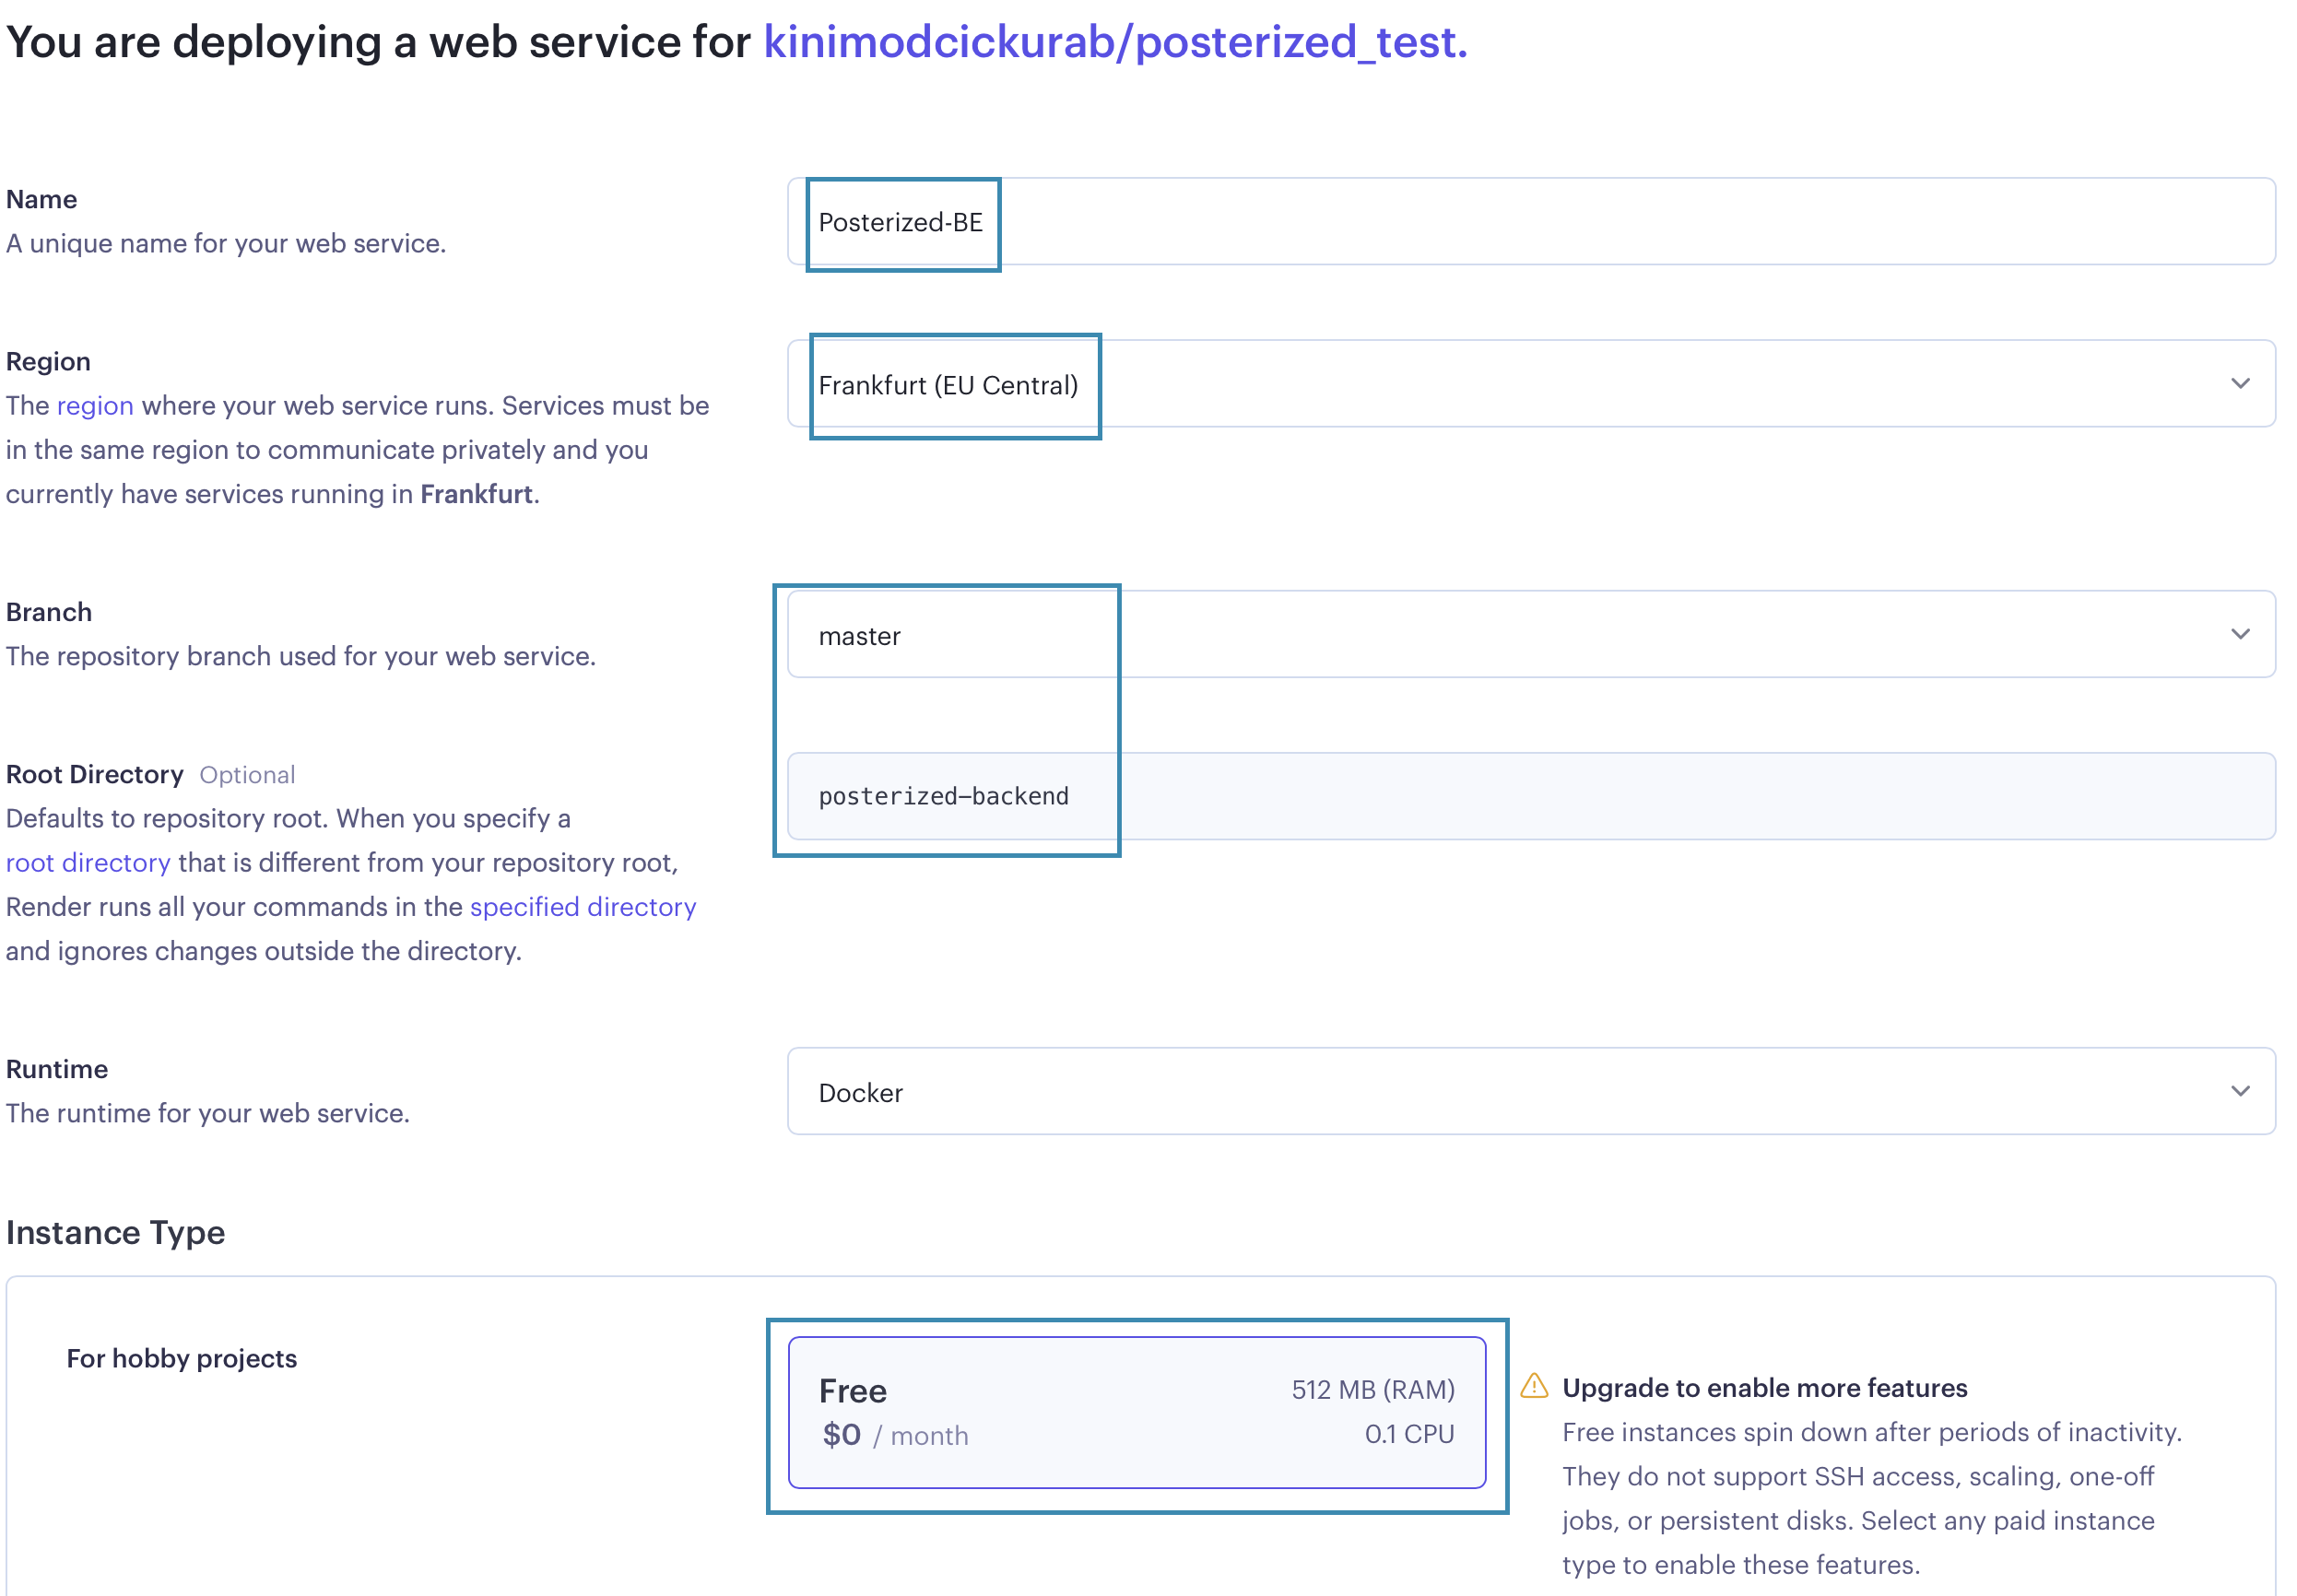
\includegraphics[scale=0.3]{slike/deploy/backend4.png} %veličina slike u odnosu na originalnu datoteku i pozicija slike
				\centering
				\caption{Kreiranje web servisa - upisivanje osnovnih podataka}
				\label{fig:promjene}
			\end{figure}
			
			Otvoriti padajući izbornik "Advanced" i upisati putanju gdje se nalazi \textit{Dockerfile}, zatim kliknuti "Create Web Service".
			\begin{figure}[H]
				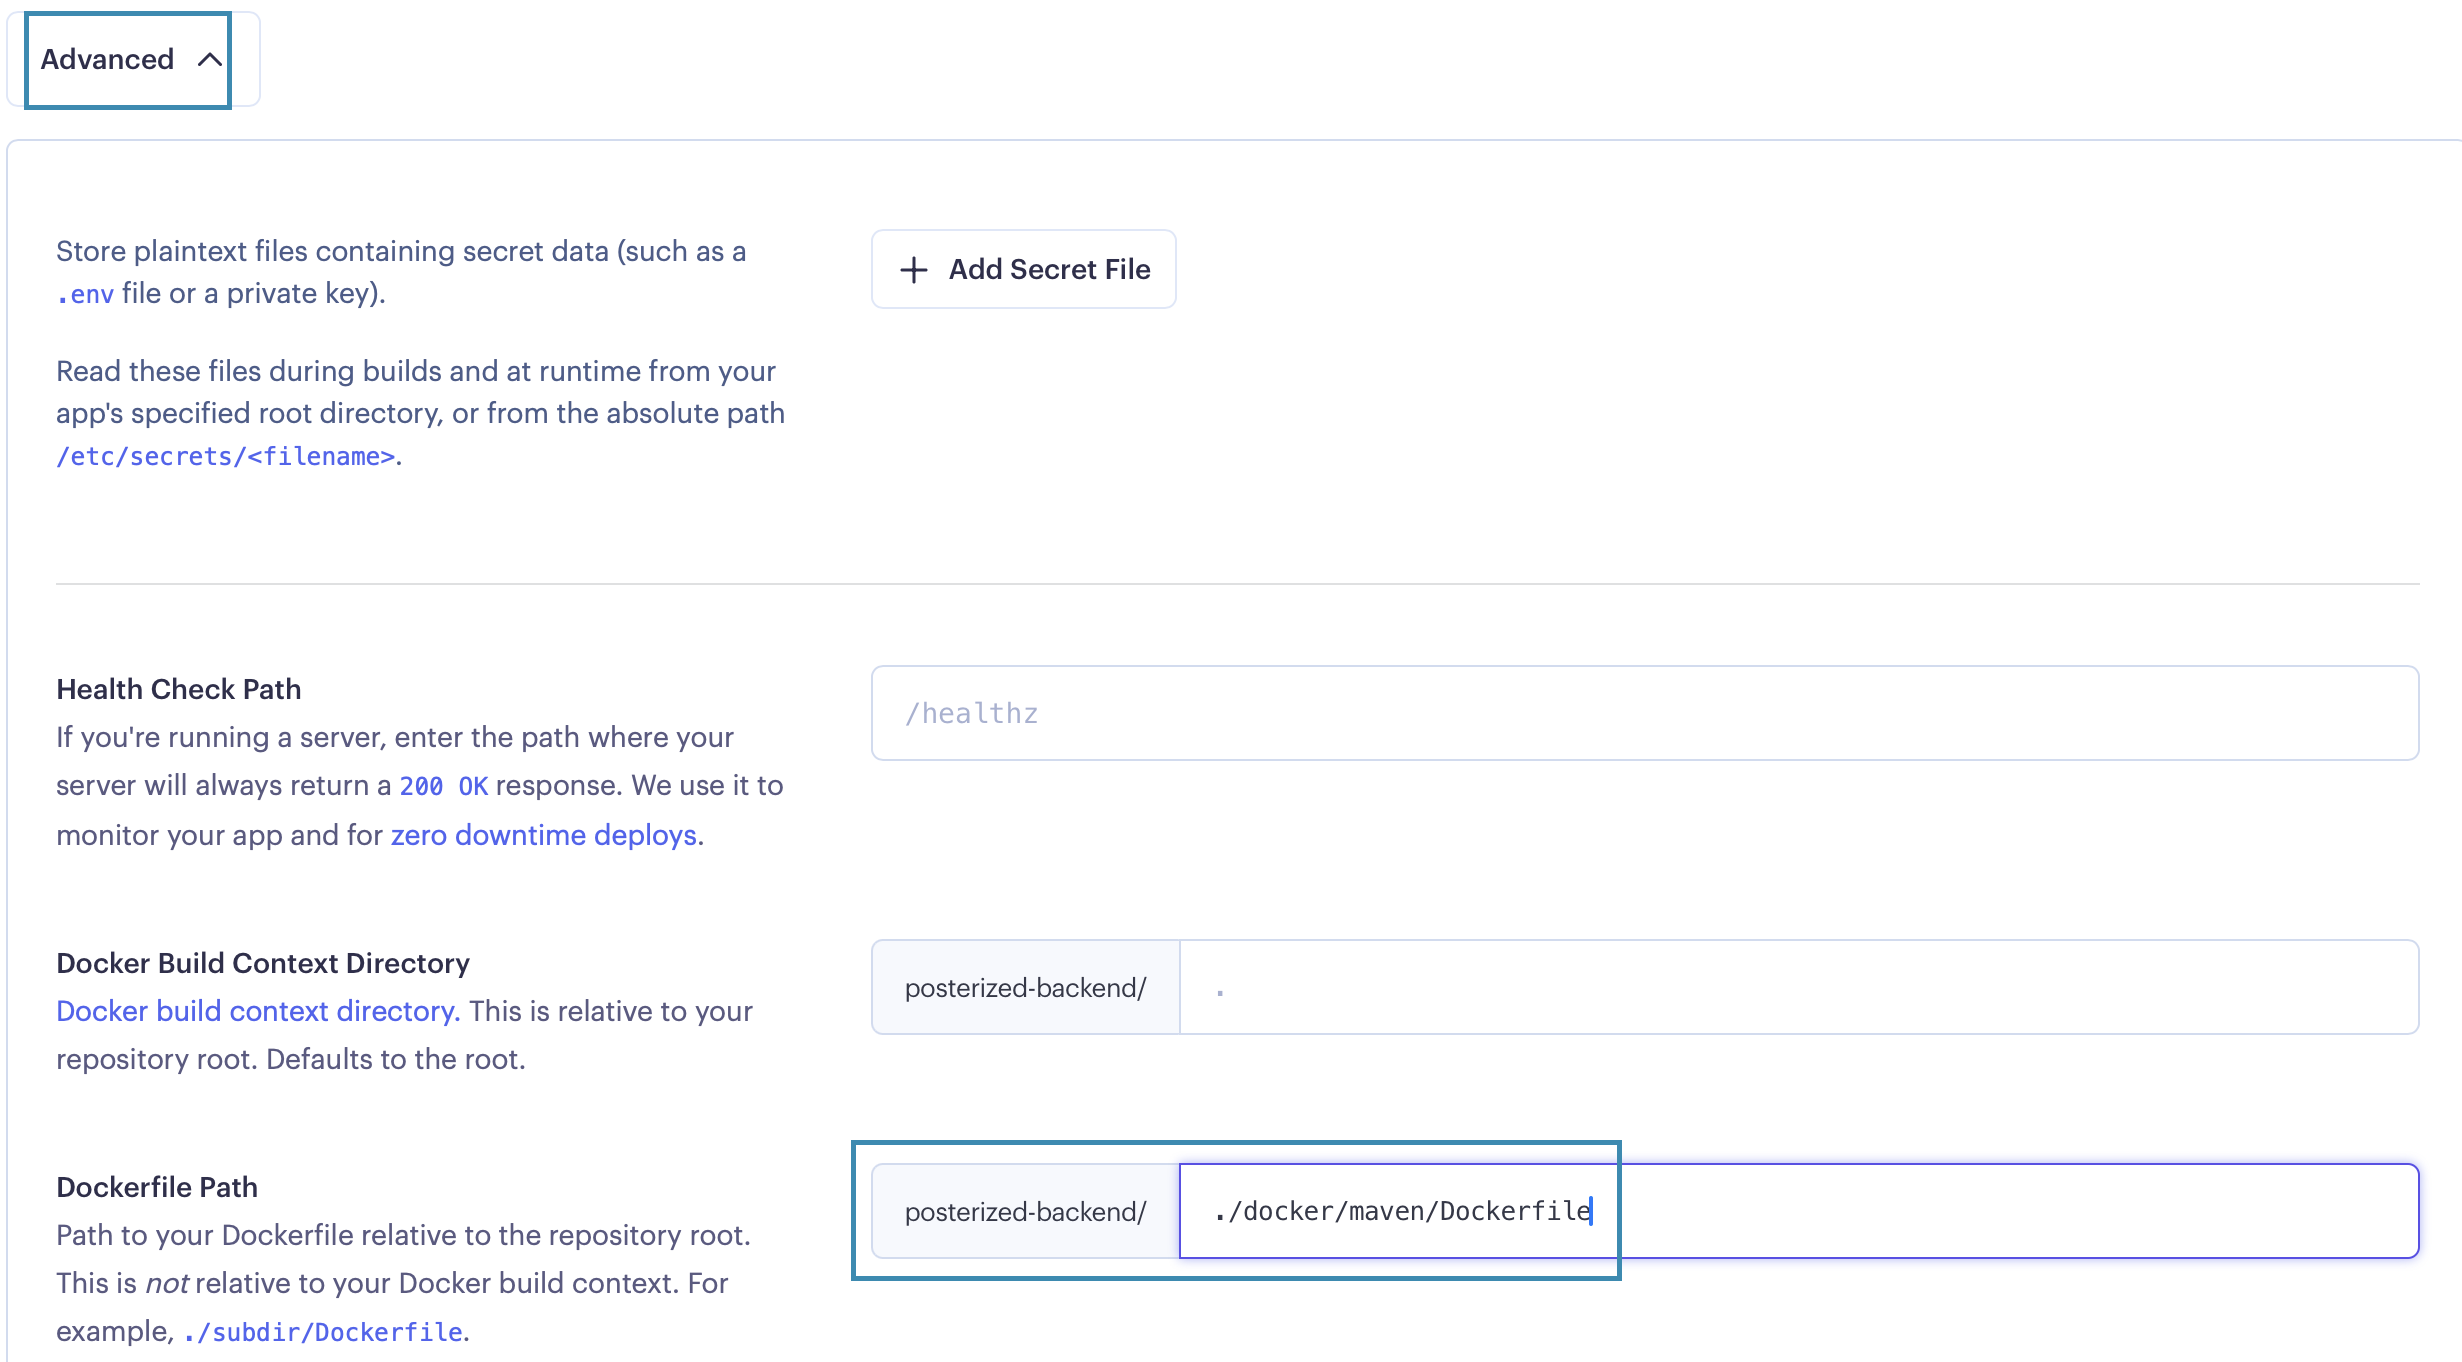
\includegraphics[scale=0.35]{slike/deploy/backend5.png} %veličina slike u odnosu na originalnu datoteku i pozicija slike
				\centering
				\caption{Navođenje \textit{Dockerfile} putanje}
				\label{fig:promjene}
			\end{figure}
			
			Web servis backenda je uspješno kreiran i pušten u pogon.
			\begin{figure}[H]
				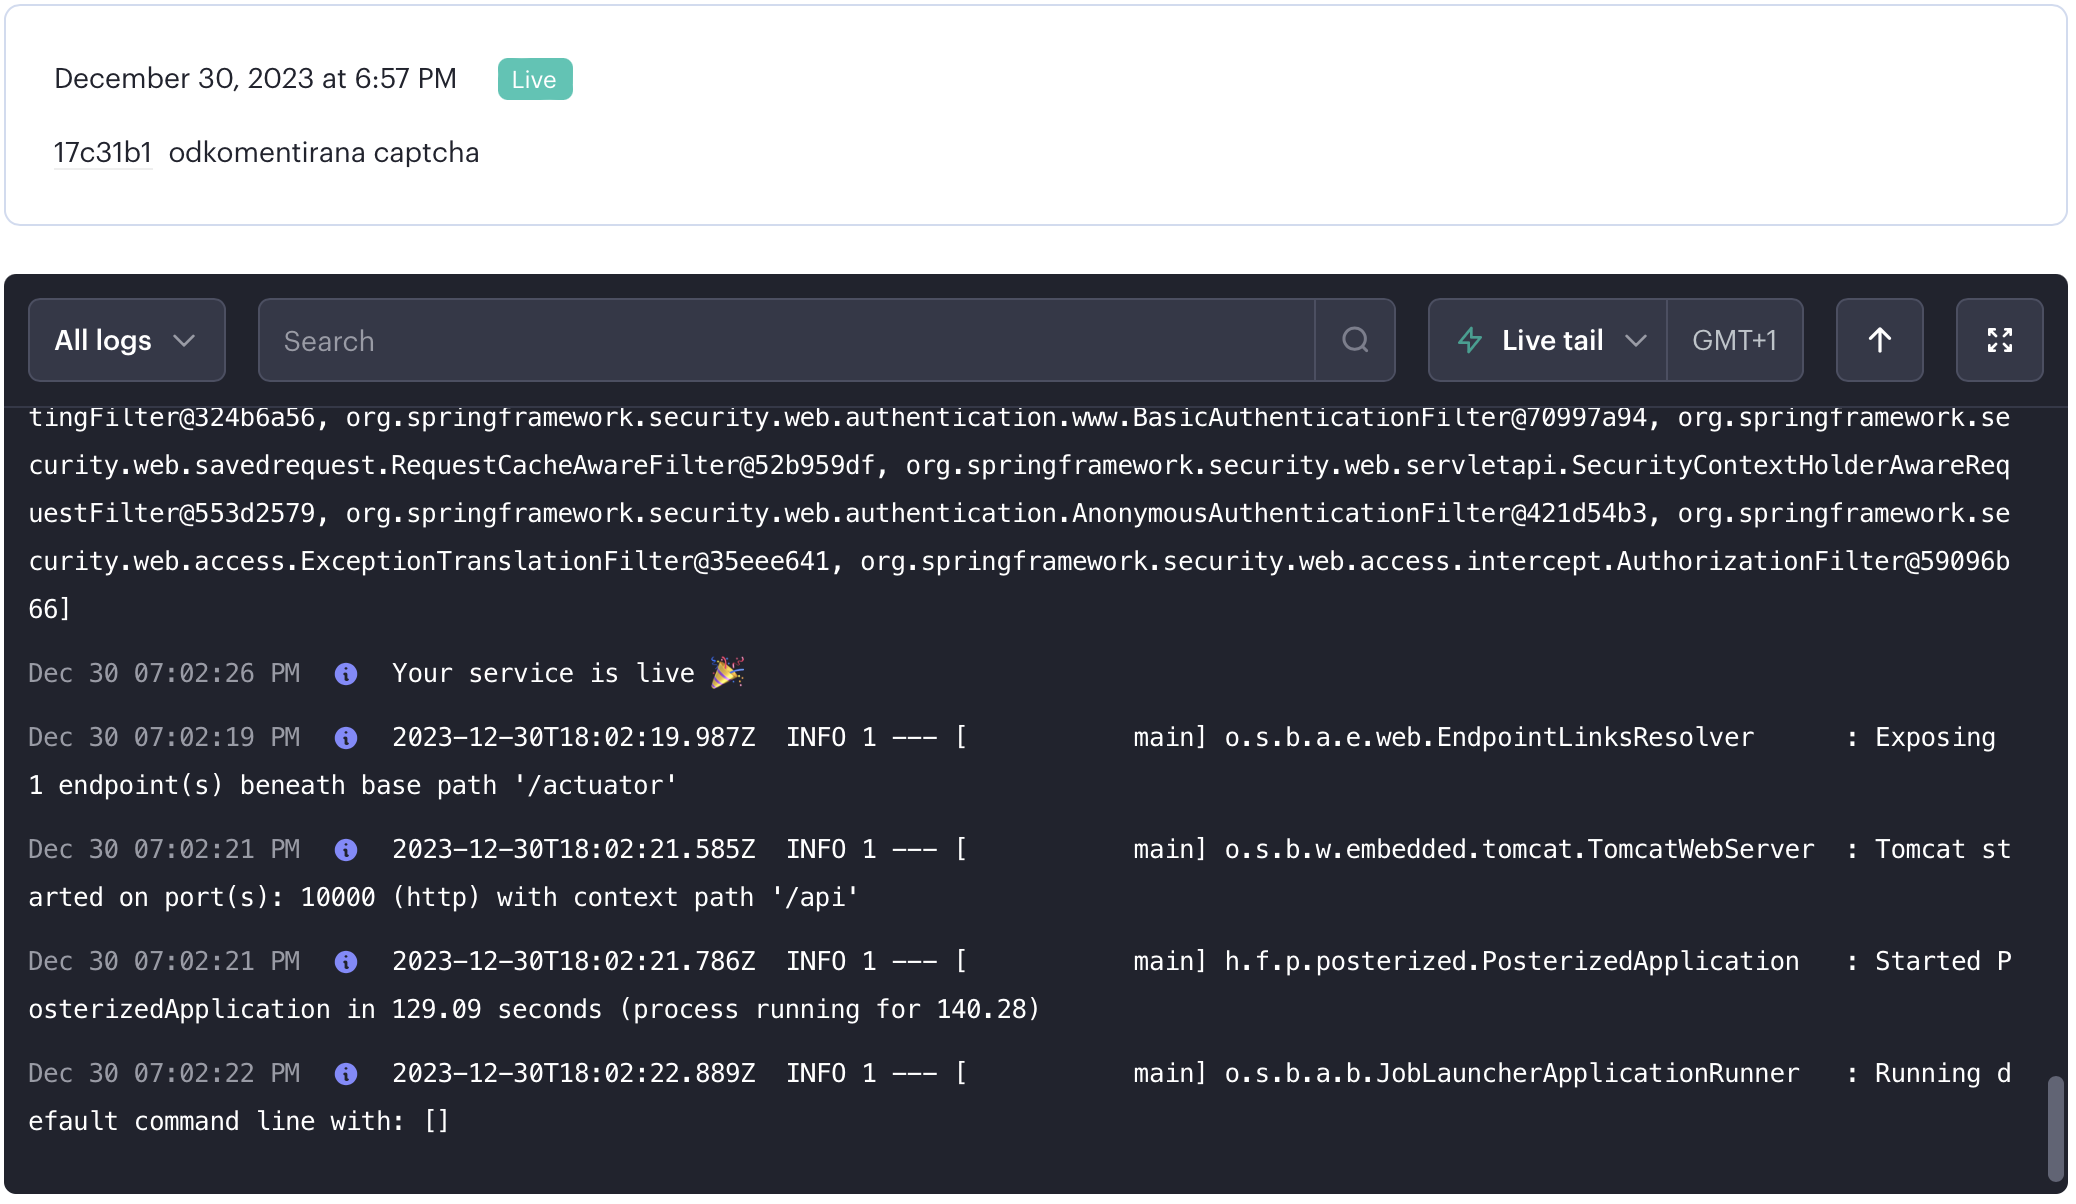
\includegraphics[scale=0.4]{slike/deploy/backend6.png} %veličina slike u odnosu na originalnu datoteku i pozicija slike
				\centering
				\caption{Logovi stvaranja i status web servisa}
				\label{fig:promjene}
			\end{figure}
			
			% za frontend
			
			
			
			\eject 